    \chapter{Popis získané datové sady a~zhodnocení výsledků}
    \label{vysledky}    
    Dále bude popsána získaná datová sada na základě provedeného experimentu. Nejprve bude popsán soubor jako celek a~poté jednotlivé signály zvolené v~podkapitole \ref{volba_zarizeni_metriky}.
    
    \section{Klíčové vlastnosti datové sady}
    
    Metriky datové sady:
    \begin{itemize}
        \item celkový počet účastníků: 16,
        \item z toho: 9 mužů, 7 žen,
        \item počet měřených emocí: 6 + klidový stav,
        \item předpokládaný počet souborů s daty: 96,
        \item výsledný počet datových souborů: 92,
        \item předpokládaný počet vzorků: 288,
        \item výsledný počet vzorků: 272,
        \item délka vzorků: $\pm$\,4 sekundy (klidový stav), 8 - 10 sekund (emoce).
    \end{itemize}
    
    Výsledný počet vzorků se liší od předpokládaného, neboť během jednotlivých sezení výjimečně docházelo k~špatnému stisku tlačítka na zařízení. V~některých případech bylo možné provést korekci a~doplnit časovou značku po skončení sezení. Doplnění probíhalo podle předešlé a~následující značky a~následného vypočítání přibližného času podle časování prezentace, při jejímž promítání chyba vznikla. V~případech, kdy nebylo možné provést korekci, musel být záznam odstraněn. Počet výsledných vzorků tvoří 94\,\% předpokládaného počtu.
    
    \subsection{Statistika}
    Datovou sadu lze rozdělit podle více kritérií: zvolená emoce, pohlaví účastníka, četnost přiřazení emoce k~jednotlivým podnětům, denní doba sezení, apod.
    
    Graf~\ref{fig:data_hist} zobrazuje výsledné rozdělení získaných dat pro jednotlivé emoce. Rozložení je nerovnoměrné, neboť volba emoce byla čistě na účastníkovi experimentu. Další aspekt ovlivňující výsledné rozložení dat je objektivita podnětů. 
    
     \begin{figure}[H]
        \centering
        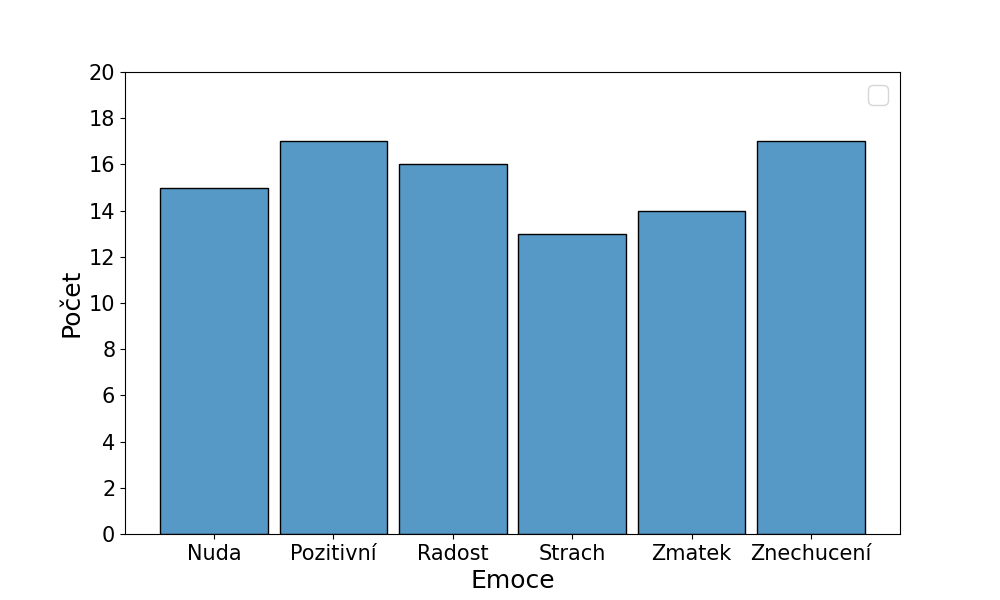
\includegraphics[width=0.85\textwidth]{obrazky-figures/hist.png}
        \caption{Histogram počtu datových záznamů pro jednotlivé emoce.}
        \label{fig:data_hist}
    \end{figure}
    
    Druhým kritériem, podle kterého jsou data rozdělena, je pohlaví účastníka experimentu. Jak ukazuje graf~\ref{fig:data_emotion_count}, je poměrně rozdílné jakou emoci jednotlivci pociťovali. Zda má vliv pohlaví účastníka na rozložení dat nelze, na základě grafu, jednoznačně určit. Proto je toto tvrzení ověřeno v~podkapitole~\ref{zhodnoceni} statistickým testem.
    
   
    \begin{figure}[H]
        \centering
        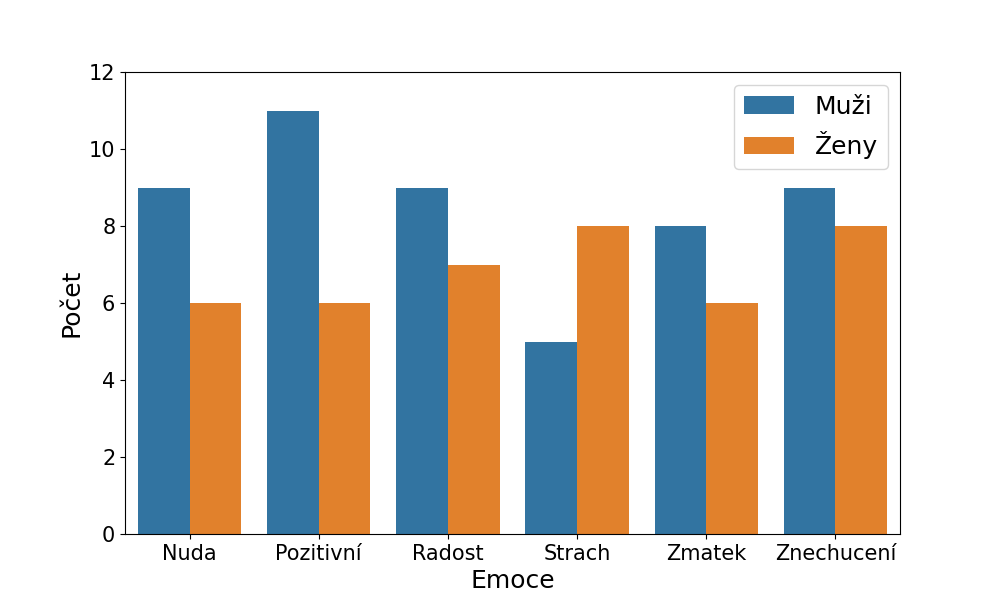
\includegraphics[width=0.85\textwidth]{obrazky-figures/emotion_count.png}
        \caption{Graf počtu datových záznamů pro jednotlivé emoce v~závislosti na pohlaví účastníka.}
        \label{fig:data_emotion_count}
    \end{figure}
    
    
    Volba emoce neprobíhala po každém podnětu, ale po malé skupině podnětů (jednotlivé prezentace). Graf~\ref{fig:heatmap_emotion_choice} zobrazuje, jak účastníci reagovali na jednotlivé prezentace.
    
    
    \begin{figure}[H]
        \centering
        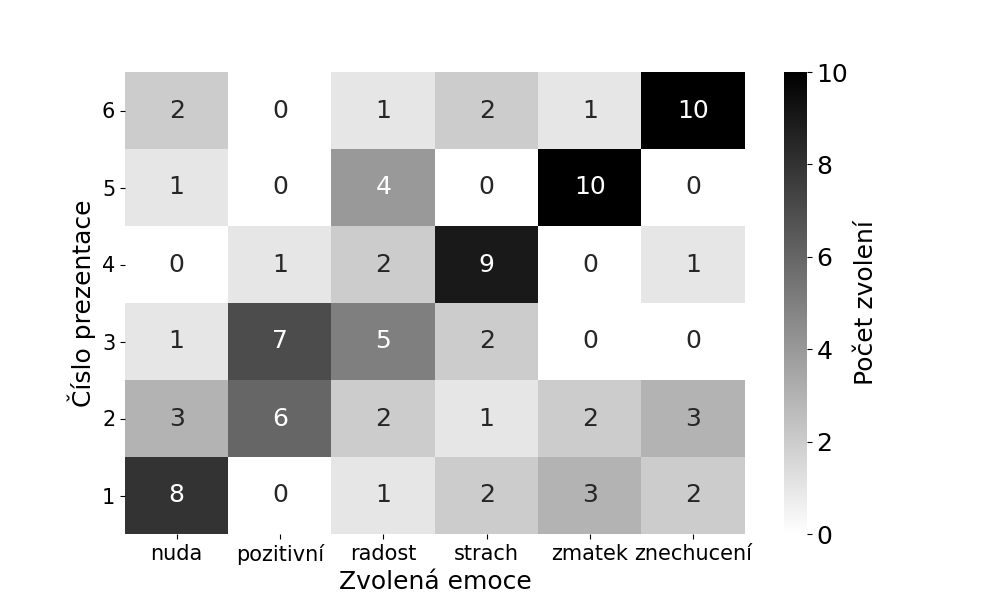
\includegraphics[width=\textwidth]{obrazky-figures/heatmap_emotion_choice.png}
        \caption{Graf četnosti přiřazení pociťované emoce k~promítané prezentaci.}
        \label{fig:heatmap_emotion_choice}
    \end{figure}
    
    Každá prezentace byla vytvořena za účelem vzbuzení konkrétní emoce. Předpoklad se zakládal na volbě jednotlivých podnětů podle kategorizačního skóre. Tím, že je nejvyšší četnost zvolené emoce na diagonále grafu, je předpoklad potvrzen. Co se týče 2.~a~3.~prezentace, není výsledek tak jednoznačný. To je způsobeno malými rozdíly mezi vybranými podněty. Jistou roli hraje také smysl pro humor člověka.
    
    \vspace{6mm}
    
    Jelikož složky s~daty obsahují v~názvu časovou značku, je poměrně snadné zpětně určit, ve kterou denní dobu bylo sezení provedeno (viz tabulka~\ref{tab:day_time}). To by mohlo být nápomocné například při zkoumání, zda má denní doba vliv na emoce člověka.
    
    \begin{table}[H]
        \centering
        \begin{tabularx}{0.8\textwidth} { 
        | >{\centering\arraybackslash}X 
        | >{\centering\arraybackslash}X 
        | >{\centering\arraybackslash}X
        | >{\centering\arraybackslash}X
        | >{\centering\arraybackslash}X |}
        \hline
        ráno & poledne & odpoledne & večer & noc \\
        \hline
        6 & 12 & 29 & 45 & 0 \\
        \hline
        \end{tabularx}
    
        \caption{Datová sada rozdělená podle denní doby, kdy bylo uskutečněno sezení. Časové intervaly jsou: ráno <4\,-\,11), poledne <11\,-\,13), odpoledne <13\,-\,18), večer <18\,-\,22), noc [<22\,-\,24), <0\,-\,4)].}
        \label{tab:day_time}
    \end{table}
    
    
    \subsection{Struktura datové sady}
    Získaná data jsou rozdělena do 3~úrovní. V~první úrovni jsou uloženy data a~jejich příznaky pro celý experiment. V~další úrovni se data člení na originální (nezpracovaná) data a~na zpracovaná. Hierarchii uložených dat zobrazuje následující strom:
    
    \vspace{6mm}
    
    \dirtree{%
    .1 data.
    .2 generická data pro všechna sezení.
    .2 složky pro jednotlivá sezení.
    .3 raw.
    .4 E4\_Bvp.
    .4 E4\_Gsr.
    .4 E4\_Hr.
    .4 E4\_Ibi.
    .4 E4\_Tag.
    .4 E4\_Temperature.
    .3 epochs.
    .4 signály rozdělené na epochy a jejich příznaky.
    .4 data pro všechny epochy pro uklidnění.
    .4 data pro všechny epochy s podněty.
    }
    
    \section{Měřené fyziologické funkce}
    Během experimentu byly měřeny tyto funkce: srdeční tep, galvanická odezva kůže a~teplota kůže. Jelikož měření probíhala v poměrně krátkých časových úsecích, teplota kůže (viz graf~\ref{fig:temp}) byla vždy téměř konstantní.
    
    \begin{figure}[H]
        \centering
        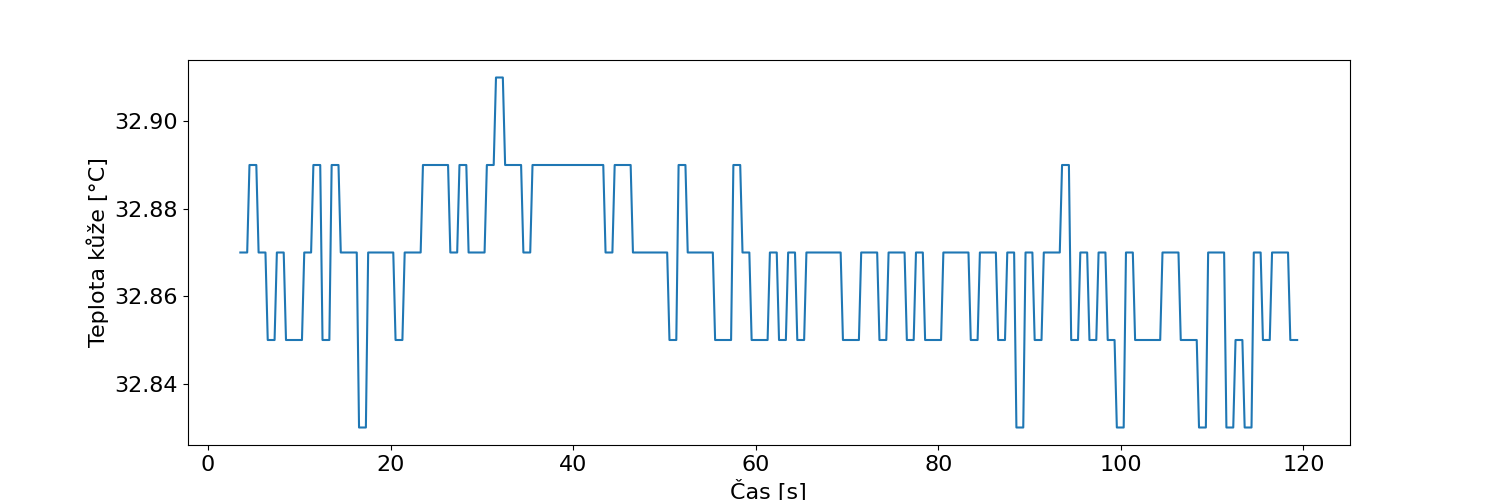
\includegraphics[width=\textwidth]{obrazky-figures/temp.png}
        \caption{Graf teploty kůže pro náhodně vybrané sezení.}
        \label{fig:temp}
    \end{figure}
    
    Z~toho důvodu je tato funkce spíše informační, nikoliv zásadní. Důležité je podotknout, že teplota kůže není rovna teplotě těla.
    
    Jako hlavní signály byly určeny PPG a EDA signál. U~těchto signálů jsou podstatné metriky (komponenty) zobrazené v~tabulce~\ref{table:priznaky_signalu}.  
    
    \begin{table}[H]
    \centering
    \begin{tabular}{ p{5cm} p{7cm}  }
        \hline
         \multicolumn{2}{c}{Podstatné komponenty signálů} \\
         \hline
         \centering
         PPG & Srdeční tep [bpm]\\
             & Variabilita srdečního tepu \\
         \hline
         \centering
         EDA & Tónická složka [$\mu$S]\\
             & Fázová reakce [$\mu$S]\\
         
         \hline
    \end{tabular}
    \caption{Tabulka příznaků měřených signálů. Jednotka bpm = beats per minute (úderů/min).}
    \label{table:priznaky_signalu}
    \end{table}
    
    Zařízení E4 poskytuje nezpracovaná i~zpracovaná data. Aby bylo možné z~nezpracovaných dat získat podstatné komponenty, musí projít jistým procesem (viz schéma~\ref{fig:signal_processing_scheme}). Proces se skládá ze tří hlavních kroků. V~prvním kroku dochází k~filtraci frekvenčního šumu. Obvykle se jedná o~vysokofrekvenční šum a~proto jsou filtry typu dolní propust. Ze vzniklého čistého signálu je již možné extrahovat příznaky signálů a~z~nich získat hodnoty hlavních komponent signálů. Datová sada obsahuje záznamy dat po každém kroku procesu.
    
    \begin{figure}[H]
        \centering
        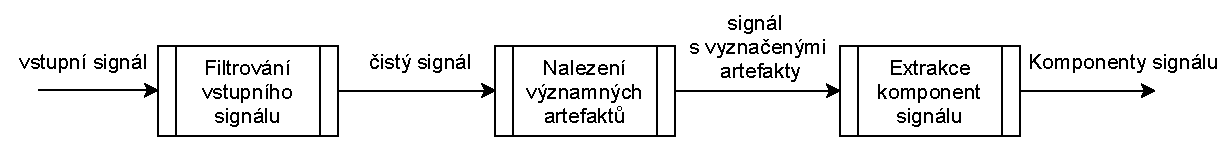
\includegraphics[width=\textwidth]{obrazky-figures/signal_processing_scheme.pdf}
        \caption{Schéma zpracování signálů během analýzy dat.}
        \label{fig:signal_processing_scheme}
    \end{figure}
    
    
    \subsection{Srdeční tep}
    Měření této fyziologické funkce probíhá pomocí PPG senzoru. PPG signál obsahuje diastolické body, z~nichž je možné vypočítat tzv. čas mezi údery (angl. Inter-Beat interval, IBI). Pomocí IBI lze následně vypočítat srdeční tep (angl. Heart Rate, HR) podle vzorce: 
    
    \begin{equation} 
        HR\,[bpm]\,= {60 / IBI}
        \label{eq:ibi_to_hr}
    \end{equation}
    
    Srdeční tep je možné získat dvěma způsoby. Zařízení E4 vysílá kromě PPG signálu, také již zpracované hodnoty IBI i~srdečního tepu. Tyto data jsou uložena pod názvem \uv{E4\_Ibi} a~\uv{E4\_Hr}. Algoritmus výpočtu srdečního tepu v~zařízení automaticky filtruje chybné vzorky. Druhou možností výpočtu srdečního tepu je vlastní výpočet. Pro ten lze využít doporučené knihovny (NeuroKit2, pyphysio). Tyto knihovny nabízí kompletní proces zpracování signálu (schéma~\ref{fig:signal_processing_scheme}). Nevýhodou však je, že obsahují i~chybná data, která algoritmus implementovaný v~zařízení nepočítá. Porovnání vypočítaných hodnot knihovnou NeuroKit2 s~hodnotami vypočítanými zařízením E4 zobrazuje graf~\ref{fig:e4_vs_nk_good}. Z~grafu je patrné, v~kterých časových úsecích jsou data nepoškozená. V~těchto úsecích hodnoty získané oběma způsoby téměř korespondují. V~úsecích, kde došlo k~zašumění dat, obsahuje signál vypočítaný nástroji knihovny NeuroKit2 velmi rychlé změny hodnot.
    
    \begin{figure}[H]
        \centering
        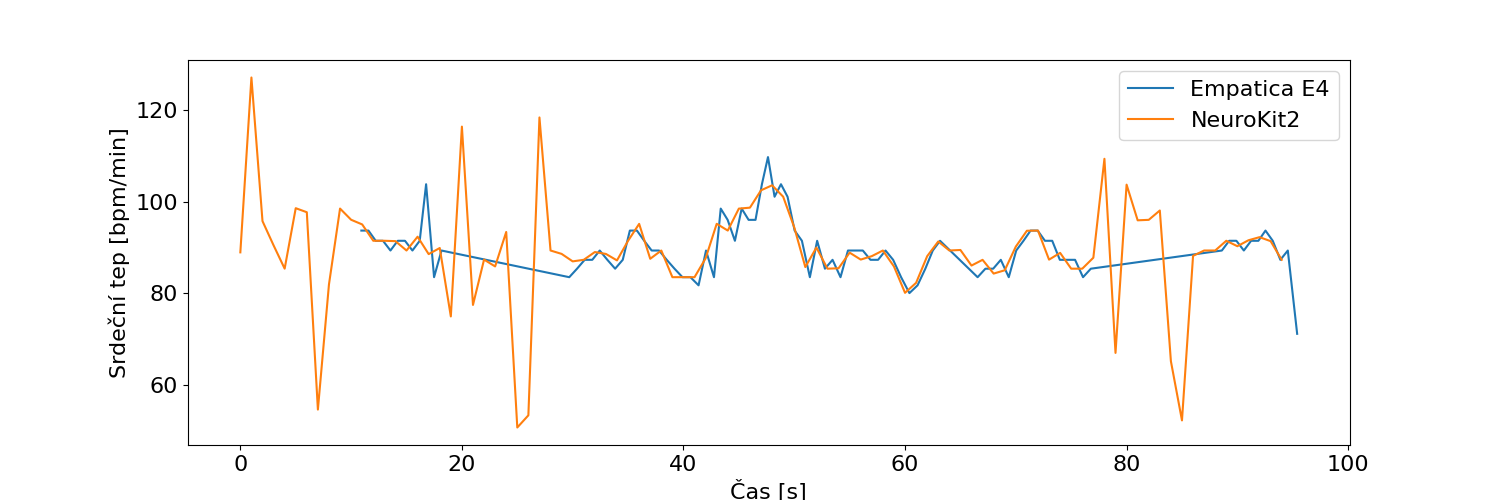
\includegraphics[width=\textwidth]{obrazky-figures/e4_vs_nk_good.png}
        \caption{Graf porovnávající vypočítané hodnoty zařízením E4 s~hodnotami vypočítanými knihovnou NeuroKit2.}
        \label{fig:e4_vs_nk_good}
    \end{figure}
    
    Díky IBI poskytovanému zařízením lze snadno určit kvalitu naměřených dat. Jelikož jsou data ve formátu <časová značka, délka vlny>, vypadá výpočet následovně: 
    
    \begin{equation} 
        if (t1 + d1) < t2:
            miss = t2 - t1 - d1
        \label{eq:miss_ratio}
    \end{equation}
    
    Kde \emph{t1} značí hodnotu časové značky kdy byla zaznamenána správná vlna, \emph{d1} značí délku této vlny a~\emph{t2} je čas první následující vlny, jenž byla validní. Hodnota \emph{miss} značí délku signálu, kdy byl poškozen. Chybovost je vyjádřena jako poměr součtu délek chybných dat ku celkové délce signálu. Chybovost pro jednotlivé emoce zobrazuje tabulka~\ref{tab:ppg_miss_ratio}. Celková chybovost dosahuje v průměru 45\%.
    
    \begin{table}[H]
        \centering
        \begin{tabularx}{0.9\textwidth} { 
        | >{\centering\arraybackslash}X 
        | >{\centering\arraybackslash}X 
        | >{\centering\arraybackslash}X
        | >{\centering\arraybackslash}X
        | >{\centering\arraybackslash}X
        | >{\centering\arraybackslash}X |}
        \hline
        nuda & pozitivní & radost & strach & zmatek & znechucení \\
        \hline
        45\,\% & 50\,\% & 41\,\% & 42\,\% & 38\,\% & 49\,\% \\
        \hline
        \end{tabularx}
    
        \caption{Chybovost naměřených dat pomocí PPG senzoru pro jednotlivé emoce.}
        \label{tab:ppg_miss_ratio}
    \end{table}
    

    \vspace{3mm}
   
   
    IBI lze také využít pro výpočet variability srdečního tepu (angl. Heart Rate Variability, HRV). Jak název napovídá, HRV značí proměnlivost časových úseků mezi dvěma údery srdce. Výpočet probíhá v klouzavých oknech. Při jeho zkoumání jsou podstatné tři složky: frekvenční (Frequency-domain features, FDF), časová (Time-domain features, TDF), nelineární (Nonlinear-domain features, NTF). Pro výpočet jsou využity opět nástroje knihovny NeuroKit2.

    
    \subsection{Galvanická odezva kůže}
    V~náramku E4 není implementovaný žádný algoritmus pro zpracování galvanické odezvy kůže, tudíž nejsou k~dispozici žádná referenční data. V~EDA signálech jsou zásadní dvě složky (tónická, fázická). Nutno zmínit, že výhodou EDA oproti PPG je větší odolnost vůči vnějším vlivům (pohyb ruky apod).
    
    Navržené knihovny poskytují nástroje pro detekci obou složek. V~této práci byla zvolena knihovna NeuroKit2. Příklad výstupních signálů zobrazuje graf~\ref{fig:tonic_phasic}. Tónická složka je zobrazena jako interpolace původního signálu a~fázická složka je normalizovaná k~nule.
    
    \begin{figure}[H]
        \centering
        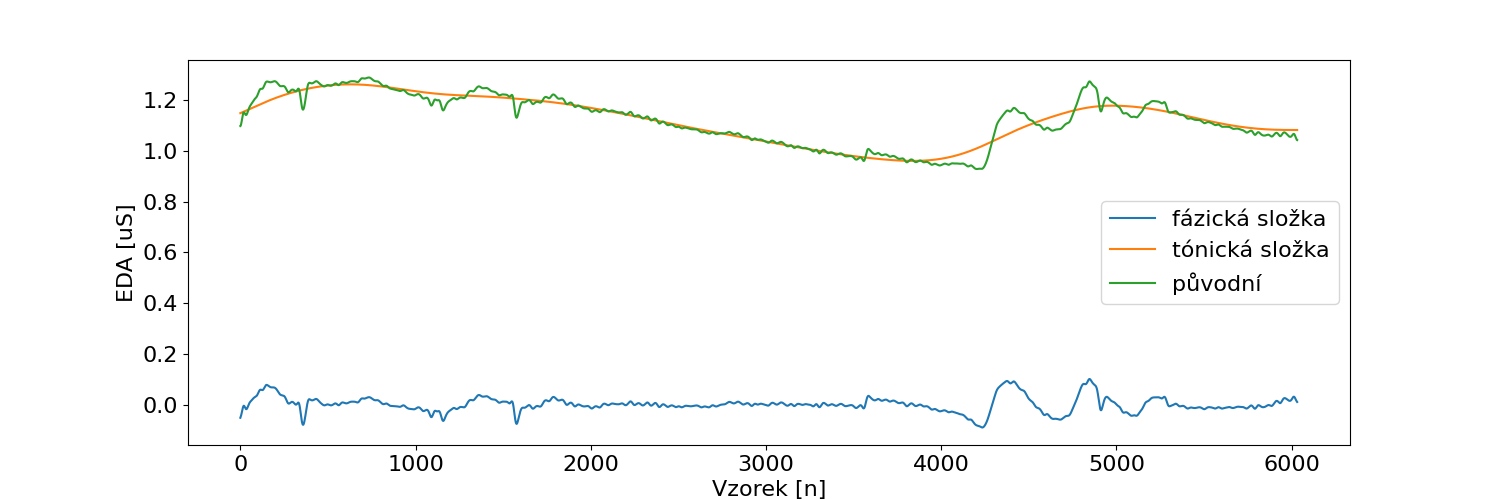
\includegraphics[width=\textwidth]{obrazky-figures/tonic_phasic.png}
        \caption{Graf zobrazující podstatné komponenty náhodně vybraného EDA signálu včetně původního.}
        \label{fig:tonic_phasic}
    \end{figure}
    
    \vspace{6mm}
    
    \subsection{Propojení hlavních komponent signálů}
    
    Výsledný graf (viz~\ref{fig:rate_vs_phasic}) dvou základních komponent (časová složka HRV, fázická složka EDA) signálů zobrazuje rozložení středních hodnot komponent ve vztahu k~jednotlivým emocím. 
    
    \begin{figure}[H]
        \centering
        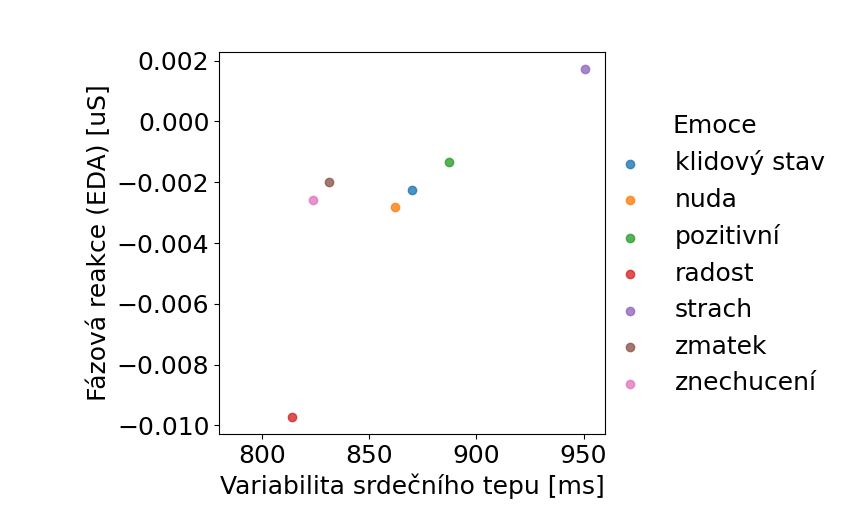
\includegraphics[width=\textwidth]{obrazky-figures/hrv_vs_phasic.png}
        \caption{Graf průměrných hodnot dvou základních komponent signálů.}
        \label{fig:rate_vs_phasic}
    \end{figure}
    
    Podle provedených studií (obecné studie:~\ref{emotion_to_physio}, studie pro zvolené zařízení:~\ref{empatica_e4}) se předpokládal pokles EDA pro neutrální podněty a~vzrůst pro pozitivní i~negativní emoce. Tento předpoklad se příliš nepotvrdil, neboť pro silně pozitivní emoci (radost) došlo k~poklesu a~pro znechucení (silnější negativní emoce) nedošlo k~výrazné změně. Předpoklad potvrdil jen strach, kdy došlo opravdu ke zvýšení EDA. Nicméně lze nahlížet na tento fakt z~jiného pohledu. Jelikož podstoupení takového experimentu vyvolává mírný stres, mohlo při pocítění radosti dojít k~většímu uvolnění testované osoby, což by vysvětlovalo výrazný pokles EDA. 
    
    Co se týče variability srdečního tepu, předpokládalo se zkrácení času mezi údery (IBI) u~silných emocí (radost, strach, znechucení, zmatek) a~naopak prodloužení, či malé změny, pro méně intenzivní emoce (nuda, pozitivní). Předpoklad potvrdily všechny emoce vyjma strachu. Nutno brát v~potaz, že vzhledem k~chybovosti PPG signálu mohlo dojít ke zkreslení výsledných hodnot HRV.
    
    \section{Zhodnocení výsledků}
    \label{zhodnoceni}
    Před začátkem experimentu byly stanoveny hypotézy o~získaných datech (viz~\ref{cil_experimentu}).
    
    \vspace{3mm}
    
    \textbf{Ověření hypotézy~1:} Bylo předpokládáno, že získaný počet vzorků pro každou emoci bude přibližně stejný. Tento předpoklad potvrzuje graf~\ref{fig:data_hist}, kde je průměrný počet vzorků na emoci~15,3 a~směrodatná odchylka~1,6. Avšak graf volby emocí k~jednotlivým prezentacím~(viz~\ref{fig:heatmap_emotion_choice}) ukazuje mírnou odchylku od předpokladu. Aby bylo možné zcela potvrdit tuto hypotézu, bylo by nutné provést experiment s~početnější testovací skupinou.
    
    \vspace{3mm}
    
    \textbf{Ověření hypotézy~2:} Zda má vliv na rozložení dat pohlaví účastníka, bylo ověřeno statistickým F--testem\footnote{\url{https://cs.wikipedia.org/wiki/F-test}} pomocí knihovny SciPy\footnote{\url{https://docs.scipy.org/doc/scipy/reference/generated/scipy.stats.f_oneway.html}}. V~testu byla určena hladina významnosti $\alpha$\,=\,0.05. Aby byla hypotéza~2 potvrzena, musí platit nerovnost: p--hodnota\footnote{\url{https://portal.matematickabiologie.cz/index.php?pg=aplikovana-analyza-klinickych-a-biologickych-dat--biostatistika-pro-matematickou-biologii--uvod-do-testovani-hypotez--p-hodnota-a-jeji-interpretace}} $< \alpha$.  Jelikož výsledná p--hodnota testu byla rovna~0.89, nebyl předpoklad potvrzen a~nedá se říci, že pohlaví účastníka má vliv na rozložení dat. 
    
    \vspace{3mm}
    
    \textbf{Ověření hypotéz~3,~4:} Jestli existuje podobnost v~naměřených datech ukazuje graf~\ref{fig:rate_vs_phasic}, kde jsou zobrazeny hlavní komponenty signálů. Střední hodnoty těchto komponent naznačují rozlišnost mezi jednotlivými emocemi. Ačkoliv rozmístění značek potvrzuje vliv síly emoce na fyziologické funkce člověka, nesplňuje rozložení předpoklady. Možný důvod byl zmíněn v~předešlé podkapitole.
    
    \vspace{3mm}
    
    \textbf{Ověření hypotézy~5:} Tato hypotéza se týká především dat získaných PPG senzorem, neboť senzor EDA je více odolný okolním vlivům, vliv má také nižší frekvence měření. Kvalita dat z~PPG senzoru byla ověřena pomocí signálu IBI vypočítaného samotným zařízením E4. Průměrná kvalita všech naměřených dat dosahuje pouze~55\,\%. Byla předpokládána správnost dat, podle dřívějších studií, alespoň~80\,\%. Tento předpoklad tedy nebyl splněn. 
    
    \vspace{3mm}
    
    
    Výsledky zpracování dat ukázaly, že zásadním aspektem je objektivita vybraných podnětů. Ačkoliv byl výběr založen na kategorizačním skóre, jedná se stále o~statistické hodnoty. Řešením by mohl být průzkum při návrhu experimentu. Průzkum lze založit na dotazníku, jenž by zkoumal emotivitu budoucích účastníků experimentu. Takový průzkum by odhalil jaké emoce účastníci prožívají nejvíce i~na základě jakých podnětů pociťují nejčastěji takové emoce. Tento postup by snížil míru objektivity a~potenciálně mohl zlepšit výsledky celého experimentu.
    
    Vliv na získaná data mělo také zvolené zařízení. Jelikož probíhalo měření co nejméně rušivou, neinvazivní metodou, obsahují data více chyb. Aby k~těmto chybám docházelo méně, lze měřit data paralelně (více zařízení najednou). Nutno podotknout, že chyba se týkala především PPG senzoru. 
    
    I~přes to, že byla data méně kvalitní, podařil se potvrdit rozdílný vliv emocí na fyziologické funkce člověka a tím také potvrdit správnost postupu při návrhu experimentu. Rozšířením práce by mohl být klasifikátor, kde by získaná datová sada sloužila jako trénovací data. Jako další rozšíření lze uvažovat jemnější kategorizaci pocítěné emoce, příkladem je metoda SAM.  
    
    
    
    
    
   
    
    
    
    